\documentclass{beamer}
\usetheme{ConnectivityLab}
\usepackage{times}
\usepackage{graphicx}
\usepackage{verbatim}
\usepackage{outlines}
\usepackage{fancyhdr}
\usepackage{subfigure}
\usepackage{cancel}
\usepackage{bibentry}
\usepackage{varwidth}
\usepackage{etoolbox}
\usepackage{epstopdf}

%%%%%%%%%%%%%%%%%%%%%%%%%%%%%%%%%%%%%%%%%%%%%%%%%%%%%%
%%%%%%%%%%%%%%%%%%%%%%%%%%%%%%%%%%%%%%%%%%%%%%%%%%%%%%

\title {
    Retransmission-based Access Class Barring for RAN overload control in Machine Type Communications
}
\author {
    Yin-Hong, Hsu
}
\date {
    09 26, 2016
}

%%%%%%%%%%%%%%%%%%%%%%%%%%%%%%%%%%%%%%%%%%%%%%%%%%%%%%
%%%%%%%%%%%%%%%%%%%%%%%%%%%%%%%%%%%%%%%%%%%%%%%%%%%%%%

\begin{document}
\begin{frame}
    \titlepage
\end{frame}

%%%%%%%%%%%%%%%%%%%%%%%%%%%%%%%%%%%%%%%%%%%%%%%%%%%%%%
%%%%%%%%%%%%%%%%%%%%%%%%%%%%%%%%%%%%%%%%%%%%%%%%%%%%%%

\begin{frame}{Outline}
    \tableofcontentsgather
    \tableofcontents
\end{frame}

%%%%%%%%%%%%%%%%%%%%%%%%%%%%%%%%%%%%%%%%%%%%%%%%%%%%%%
%%%%%%%%%%%%%%%%%%%%%%%%%%%%%%%%%%%%%%%%%%%%%%%%%%%%%%
\section{Aim}

%%%%%%%%%%%%%%%%%%%%%%%%%%%%%%%%%%%%%%%%%%%%%%%%%%%%%%
%%%%%%%%%%%%%%%%%%%%%%%%%%%%%%%%%%%%%%%%%%%%%%%%%%%%%%
\begin{frame} {Aim} 
    \begin{itemize}
        \item \textbf{In order to alleviate the RAN overload,}
        \item [-]{We focus on the objective that can increase access success probability and relieve the access delays.}
        \item \textbf{Accroding to traditional ACB factor is fixed.}
        \item [-]{We proposed an algorithm to make eNB be able to change ACB factor dynamically.} 
    \end{itemize}
\end{frame}

%%%%%%%%%%%%%%%%%%%%%%%%%%%%%%%%%%%%%%%%%%%%%%%%%%%%%%
%%%%%%%%%%%%%%%%%%%%%%%%%%%%%%%%%%%%%%%%%%%%%%%%%%%%%%
\section{Background}
\begin{frame}{Background}
\begin{itemize}
    \item \textbf{Random Access Procedure}
    \begin{itemize}
        \item [-]{When UE device is switched on or handover from on eNB to another.}
        \item[-]{UEs will contend resource blocks with others.}
        \item[-]{Is classified into two type in LTE, contend based and contend free.}
    \end{itemize}
\end{itemize}

\end{frame}
\begin{frame}{Background}
    \begin{itemize}
    \item{4 step in random access procedure}
    \end{itemize}
    \begin{figure}[t]
        \centering
        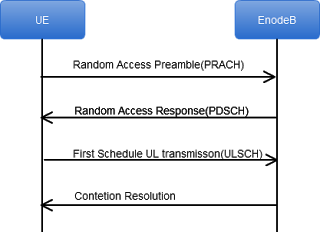
\includegraphics[width=0.6\textwidth]{figures/rach.png}
        \setbeamerfont{caption}{size=\tiny}
        \caption{RAP}
    \end{figure}
\end{frame}

%%%%%%%%%%%%%%%%%%%%%%%%%%%%%%%%%%%%%%%%%%%%%%%%%%%%%%
%%%%%%%%%%%%%%%%%%%%%%%%%%%%%%%%%%%%%%%%%%%%%%%%%%%%%%
\section{System model}
\begin{frame}{{System model}\\Random Access Procedure}
    \begin{itemize}
        \item{Devices will receive info from SIB2}
        \item{Device will choose a preamble and increase preamble transmission}
        \begin{itemize}
            \item[-] wait for Random Access Response(Msg2)
            \item[-] if fail to receive RAR, it will wait for a backoff time to retry if the times of transmission is smaller than maximum
        \end{itemize}
        \item{Sending the connection request(Msg3)}
        \begin{itemize}
            \item[-]{If successfully to transmit the preamble to eNB, it will finish the RAP}
            \item[-] if it fail to receive contend resolution(Msg4), it will wait for a backoff time to retry if the times of transmission is smaller than maximum
        \end{itemize}
    \end{itemize}
\end{frame}
\begin{frame}{{System model}\\Random Access Procedure}
    \begin{figure}[t]
        \centering
        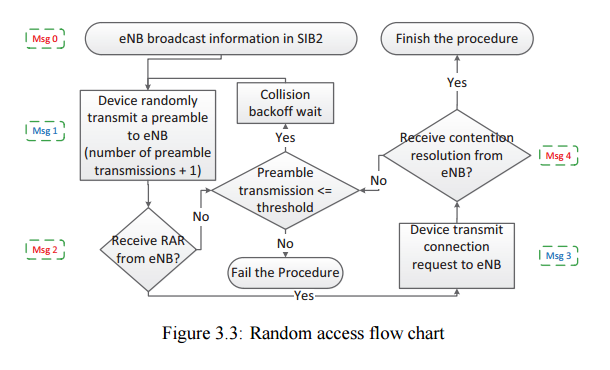
\includegraphics[width=0.9\textwidth]{figures/3_3.png}
        \setbeamerfont{caption}{size=\tiny}
        \caption{RAP flow chart}
    \end{figure}
\end{frame}
\begin{frame}{{System model}\\Access Class Barring Scheme}
    \begin{figure}[t]
        \centering
        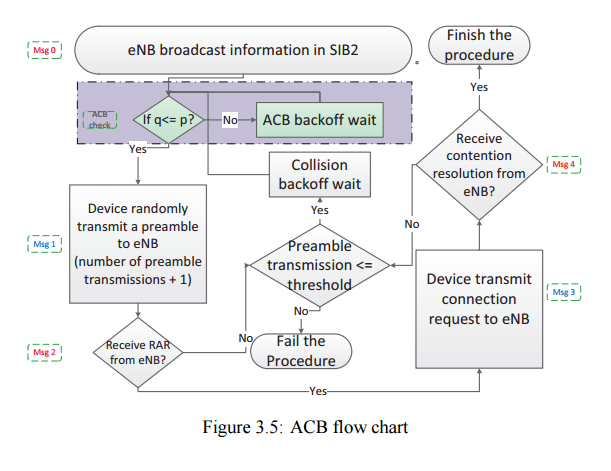
\includegraphics[width=0.6\textwidth]{figures/3_4.png}
        \setbeamerfont{caption}{size=\tiny}
        \caption{add ACB check in rap flow}
    \end{figure}
\end{frame}
\begin{frame}{{System model}\\Access Class Barring Scheme}
    \begin{itemize}
        \item{ACB factor is broadcasted by eNB}
        \item{Each device yield a random value q, if q  less than p, it passed the check of ACB and allowed to perform RAP}
        \item If not, it will be barred and wait for a backoff time of ACB to retry.
    \end{itemize}
\end{frame}

\begin{frame}{{System model}\\Performance Metric}
    \begin{itemize}
        \item Access success probability
        \begin{itemize}
            \item[-] the probability to successfully complete the RAP within the maximum times of retransmission
        \end{itemize}
        \item Access Delay
        \begin{itemize}
            \item[-] the RACH slots between the first random access attempt and the completion.
        \end{itemize}
    \end{itemize}
\end{frame}


\section{Retransmission based grouping ACB}
\begin{frame}{New grouping concept}
    \begin{itemize}
        \item Add a new message in SIB2 used to group devices into several groups.
        \item the new message are the range of the times of preamble transmissions.
    \end{itemize}
\end{frame}
\begin{frame}{New grouping concept}
    \begin{figure}[t]
        \centering
        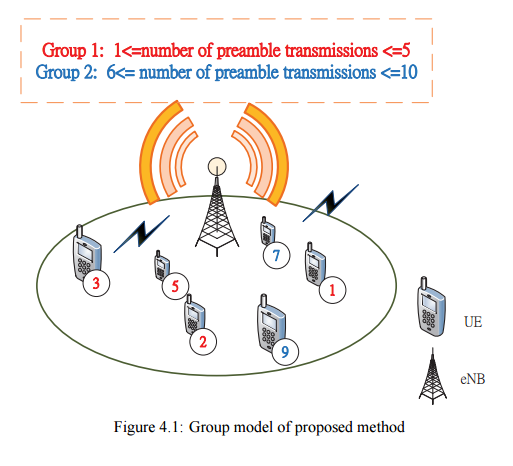
\includegraphics[width=0.8\textwidth]{figures/4_1.png}
        \setbeamerfont{caption}{size=\tiny}
    \end{figure}
\end{frame}
\begin{frame}{New grouping concept}
    \begin{itemize}
        \item We obtain it's estimation N' according to the existing information
        \begin{itemize}
            \item[-] number of success preambles and collision preambles.
            \item[-] N is all number of device that perform preamble transmission.
        \end{itemize}
        \item We let device who success to perform preamble transmission return it times of preamble transmissions in Msg3 of RAP.
    \end{itemize}
    
\end{frame}
% \begin{frame}{New grouping concept}
%     \begin{itemize}
%         \item With the information above, we can get $G^{{m}}_{{\alpha,\beta}}$, the number of devices who belong to group m and perform ${{\alpha}}$ th and ${{\beta}}$ th preamble transmission in an RACH slot.\\
%         \item With $G^{{m}}_{{\alpha,\beta}}$, we can be able to observe RAN loading and further to change ACB factor according to different loading condition.
%     \end{itemize}
% \end{frame}
\begin{frame}{New grouping concept}
    \begin{figure}[t]
        \centering
        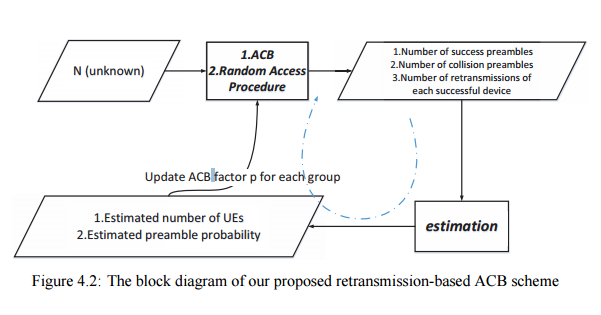
\includegraphics[width=0.9\textwidth]{figures/4_2.png}
        \setbeamerfont{caption}{size=\tiny}
    \end{figure}
\end{frame}
\begin{frame}{New grouping concept}
    \begin{figure}[t]
        \centering
        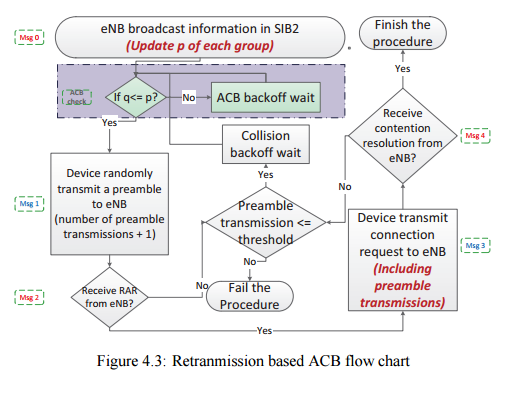
\includegraphics[width=0.9\textwidth]{figures/4_3.png}
        \setbeamerfont{caption}{size=\tiny}
    \end{figure}
\end{frame}
%%%%%%%%%%%%%%%%%%%%%%%%%%%%%%%%%%%%%%%%%%%%%%%%%%%%%%
%%%%%%%%%%%%%%%%%%%%%%%%%%%%%%%%%%%%%%%%%%%%%%%%%%%%%%
\section{Mathmatic}
\begin{frame}{Update ACB factor dynamically}
    \begin{itemize}
        \item The group which has larger threshold has higher priority.
        \begin{itemize}
            \item[-] To accomplish this; we assign each group to a different weight $w_{{m}}$
        \end{itemize}
        \item $w_{{m}}$ can be consider as the proportion of the allocation of RACH resource.
        \begin{itemize}
            \item[-] so that $\sum w_{{m}}=1$
        \end{itemize}
    \end{itemize}
\end{frame}
\begin{frame}{Update ACB factor dynamically}
    \begin{figure}[t]
        \centering
        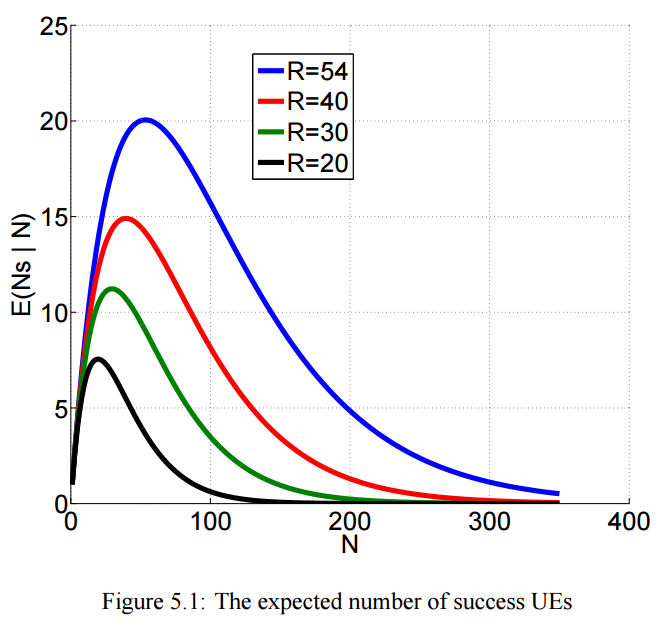
\includegraphics[width=0.7\textwidth]{figures/5_1.png}
        \setbeamerfont{caption}{size=\tiny}
    \end{figure}
\end{frame}
\begin{frame}{Update ACB factor dynamically}
    \begin{itemize}
        \item Due to the $E(N_s|N)$ be maximum while N is equal to R or R-1
        \begin{itemize}
            \item[-] we hope that there are only $N \approx R$ device who attemp to perform preamble transmission in a RACH slot. 
        \end{itemize}
        \item $P_m$ is the ACB factor of group m and R is the number of devices which passed the ACB.
        \item $p_m = \frac {W_mR}{N'}$
    \end{itemize}
\end{frame}
\begin{frame}{Update ACB factor dynamically}
    \begin{figure}[t]
        \centering
        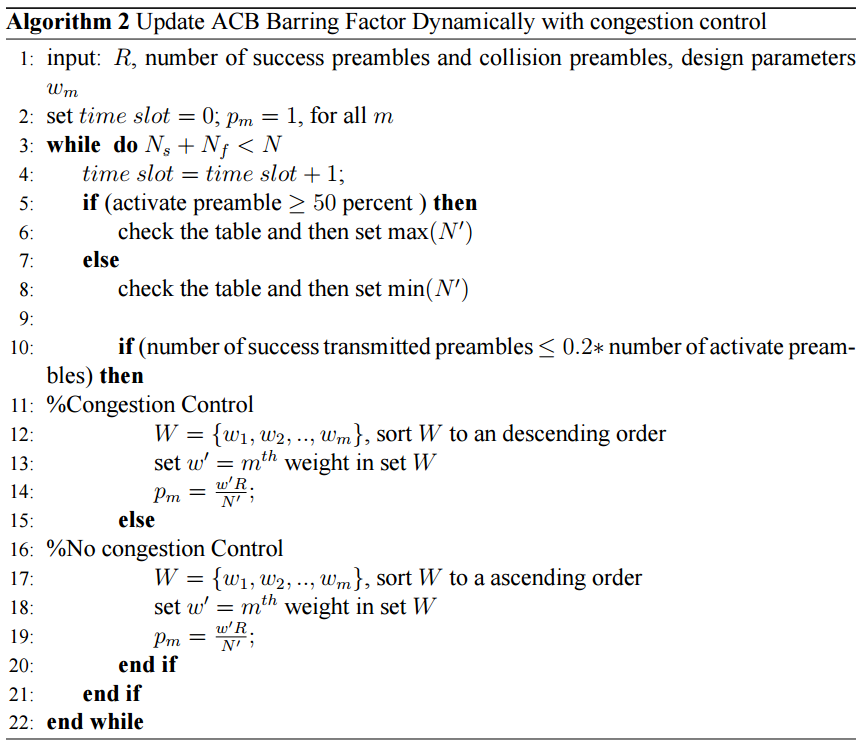
\includegraphics[width=0.7\textwidth]{figures/A_2.png}
        \setbeamerfont{caption}{size=\tiny}
    \end{figure}
\end{frame}
%%%%%%%%%%%%%%%%%%%%%%%%%%%%%%%%%%%%%%%%%%%%%%%%%%%%%%
%%%%%%%%%%%%%%%%%%%%%%%%%%%%%%%%%%%%%%%%%%%%%%%%%%%%%%
\section{Simulation Result}
\begin{frame}{Simulation Result}
    \begin{figure}[t]
        \centering
        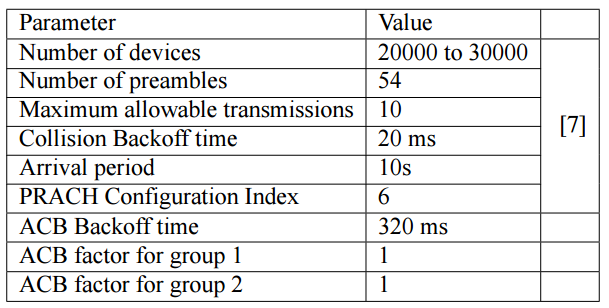
\includegraphics[width=0.9\textwidth]{figures/data.png}
        \setbeamerfont{caption}{size=\tiny}
        \caption{Simulation parameter}
    \end{figure}
\end{frame}
\begin{frame}{Simulation Result}
    \begin{figure}[t]
        \centering
        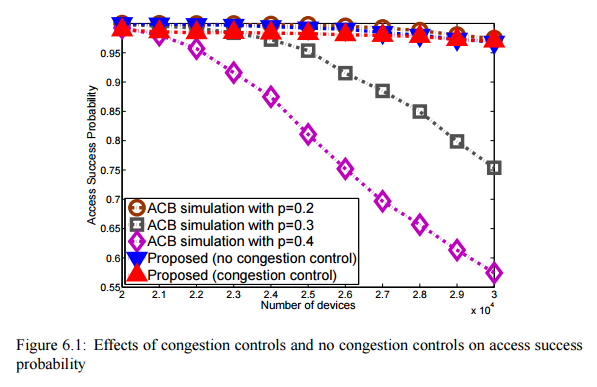
\includegraphics[width=0.9\textwidth]{figures/6_1.png}
        \setbeamerfont{caption}{size=\tiny}
    \end{figure}
\end{frame}
\begin{frame}{Simulation Result}
    \begin{figure}[t]
        \centering
        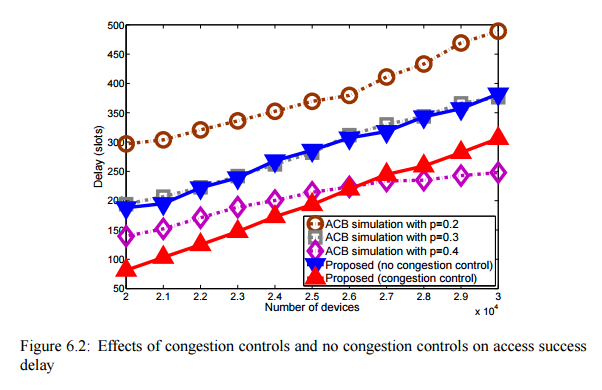
\includegraphics[width=0.9\textwidth]{figures/6_2.png}
        \setbeamerfont{caption}{size=\tiny}
    \end{figure}
\end{frame}
\begin{frame}{Simulation Result}
    \begin{figure}[t]
        \centering
        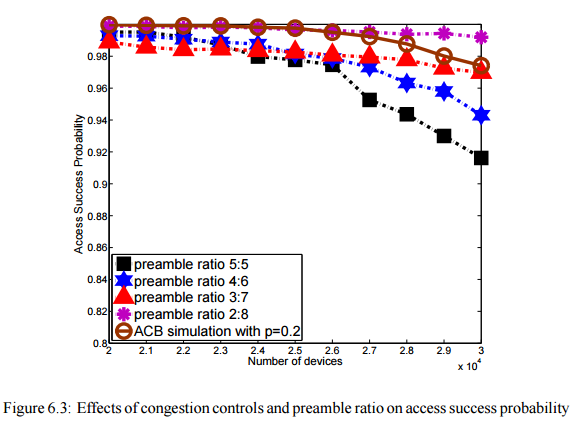
\includegraphics[width=0.9\textwidth]{figures/6_3.png}
        \setbeamerfont{caption}{size=\tiny}
    \end{figure}
\end{frame}
\begin{frame}{Simulation Result}
    \begin{figure}[t]
        \centering
        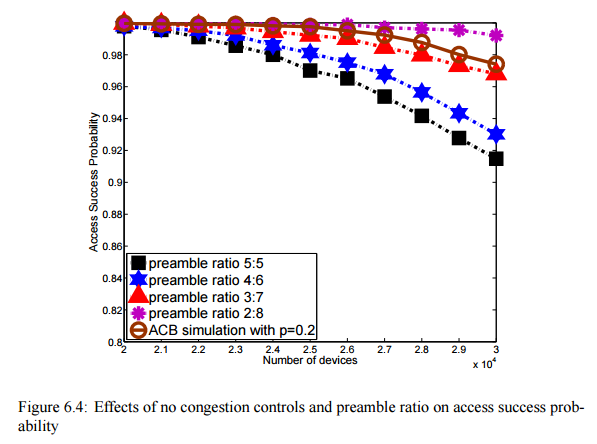
\includegraphics[width=0.9\textwidth]{figures/6_4.png}
        \setbeamerfont{caption}{size=\tiny}
    \end{figure}
\end{frame}
%%%%%%%%%%%%%%%%%%%%%%%%%%%%%%%%%%%%%%%%%%%%%%%%%%%%%%
%%%%%%%%%%%%%%%%%%%%%%%%%%%%%%%%%%%%%%%%%%%%%%%%%%%%%%
\section{References}
\calcreferencespagetotal % Calc your References Page total number
\begin{frame}[allowframebreaks]{References}
    \fontsize{9pt}{13}\selectfont
    \bibliographystyle{IEEEtran}
    \bibliography{IEEEabrv,Citation}
\end{frame}

%%%%%%%%%%%%%%%%%%%%%%%%%%%%%%%%%%%%%%%%%%%%%%%%%%%%%%
%%%%%%%%%%%%%%%%%%%%%%%%%%%%%%%%%%%%%%%%%%%%%%%%%%%%%%
\section{}

\begin{frame}
    \centering
    \Large{Thanks for Your Attentions}
\end{frame}

\end{document}
